% Copyright 2004 by Till Tantau <tantau@users.sourceforge.net>.
%
% In principle, this file can be redistributed and/or modified under
% the terms of the GNU Public License, version 2.
%
% However, this file is supposed to be a template to be modified
% for your own needs. For this reason, if you use this file as a
% template and not specifically distribute it as part of a another
% package/program, I grant the extra permission to freely copy and
% modify this file as you see fit and even to delete this copyright
% notice. 
\documentclass{beamer}

% There are many different themes available for Beamer. A comprehensive
% list with examples is given here:
% http://deic.uab.es/~iblanes/beamer_gallery/index_by_theme.html
% You can uncomment the themes below if you would like to use a different
% one:
%\usetheme{AnnArbor}
%\usetheme{Antibes}
%\usetheme{Bergen}
%\usetheme{Berkeley}
%\usetheme{Berlin}
%\usetheme{Boadilla}
%\usetheme{boxes}
%\usetheme{CambridgeUS}
%\usetheme{Copenhagen}
%\usetheme{Darmstadt}
%\usetheme{default}
\usetheme{Frankfurt}
%\usetheme{Goettingen}
%\usetheme{Hannover}
%\usetheme{Ilmenau}
%\usetheme{JuanLesPins}
%\usetheme{Luebeck}
%\usetheme{Madrid}
%\usetheme{Malmoe}
%\usetheme{Marburg}
%\usetheme{Montpellier}
%\usetheme{PaloAlto}
%\usetheme{Pittsburgh}
%\usetheme{Rochester}
%\usetheme{Singapore}
%\usetheme{Szeged}
%\usetheme{Warsaw}

\newcommand\Fontmetadata{\fontsize{8}{7.2}\selectfont}

\usecolortheme{beaver}

%\title{Presentation Title}
\title{
		{An intelligent system for churn prediction and customer retention: a case of telecommunications company }
	}

% A subtitle is optional and this may be deleted
%\subtitle{Optional Subtitle}

\author{Parth Sarangi}%\inst{1}}
% - Give the names in the same order as the appear in the paper.
% - Use the \inst{?} command only if the authors have different
%   affiliation.

\institute[Asian Institute of Technology Thailand] % (optional, but mostly needed)
{
%  \inst{1}%
  Computer Science and Information Management\\
  Asian Institute of Technology Thailand
%  \and
%  \inst{2}%
%  Department of Theoretical Philosophy\\
%  University of Elsewhere
  }
% - Use the \inst command only if there are several affiliations.
% - Keep it simple, no one is interested in your street address.

\date{Thesis Progress, September 2017}
% - Either use conference name or its abbreviation.
% - Not really informative to the audience, more for people (including
%   yourself) who are reading the slides online

\subject{Theoretical Computer Science}
% This is only inserted into the PDF information catalog. Can be left
% out. 

% If you have a file called "university-logo-filename.xxx", where xxx
% is a graphic format that can be processed by latex or pdflatex,
% resp., then you can add a logo as follows:

% \pgfdeclareimage[height=0.5cm]{university-logo}{university-logo-filename}
% \logo{\pgfuseimage{university-logo}}

% Delete this, if you do not want the table of contents to pop up at
% the beginning of each subsection:
%\AtBeginSubsection[]
%{
%  \begin{frame}<beamer>{Outline}
%    \tableofcontents[currentsection,currentsubsection]
%  \end{frame}
%}

\AtBeginSection{
	\begin{frame}<beamer>{Table of Contents}
		\tableofcontents{currentsection,currentsubsection}
	\end{frame}
	}

% Let's get started
\begin{document}

\begin{frame}
  \titlepage
\end{frame}

%------------------------------------------------Section
\section{Introduction}

\subsection{Overview}
\begin{frame}{Overview}
	\begin{itemize}
		\item Telecom industry is highly competitive
		\item Government deregulation policies
		\item Affordable handsets and Technological advancements
		\item Disruptive plans and services by rival companies
		\item Database reveals trends of service usage
		\item Data mining to identify churn customers
	\end{itemize}
\end{frame}

\begin{frame}{Overview(contd.)}
	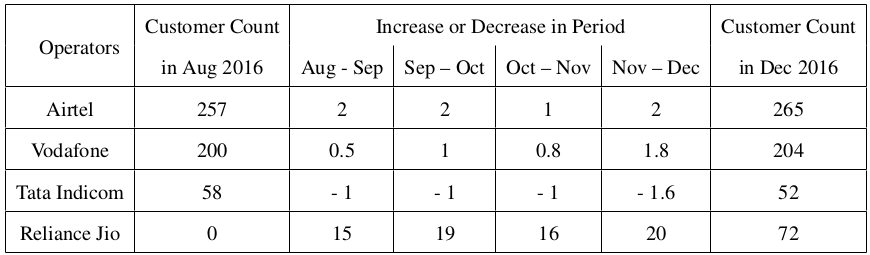
\includegraphics[scale = 0.35]{ppt_figures/introtable.png}
	\begin{itemize}
		\item TRAI - Telecom regulatory authority of India
		\item Reports subscribers at end of every month
		\item Table shows Relance Jio acquiring 72 million at end of 4 months
		\item Launch of 4G services by Jio have jolted the revenues of Airtel, Vodafone, Tata Indicom.
		\item High customer churn noticed
	\end{itemize}
\end{frame}

\subsection{Problem Statement}
\begin{frame}{Problem Statement}
	\begin{itemize}
		\item Constant product marketing by competitors
		\item Various cost effective data schemes. Night time free or high speeds, or unlimited usage plans
		\item Proactive mindset of incumbent services provider to identify unfaithful customers
		\item High investment cost of acquiring new customer
		\item Not a fully integrated system developed for churn prediction
	\end{itemize}
\end{frame}

\subsection{Objectives}
\begin{frame}{Objectives}
	\textbf{Overall objective} - develop an intelligent system for churn prediction and customer retention ICPCR.\\	
	\textbf{Specific objectives} :
	\begin{itemize}
		\item {
			Design models and evaluate prediction performance for churn.
		}
		\item {
			Build the system of intelligent churn prediction and customer retention system.
		}
		\item Evaluate the system for reliable performance.
	\end{itemize}
\end{frame}


\subsection{Limitations and Scope}
\begin{frame}{Limitations and Scope}
	\begin{itemize}
		\item {
			Many models for churn prediction.
		}
		\item Scope of this thesis is tentatively limited to build ICPCR with 3 models - Decision tree , Support Vector Machine , Artificial Neural Network
	\end{itemize}
\end{frame}

%------------------------------------------------Section
\section{Literature Review}
%

\subsection{Customer Churn \& Retention}
\begin{frame}{Customer Churn \& Retention}
	\begin{itemize}
		\item In the research paper it was found that Companies profit if they can retain customer
		\item Customers are most valuable asset.
		\item Long serving customers influence new customers to buy contracts
		\item Average Revenue Per User ARPU for telecom company is high if a customer stays
		\item If customers churn there is a loss of revenue
		\item Also acquiring new customer is expensive
		\item Forbes predicted a 10\% swing in revenue if customers are retained
	\end{itemize}
\end{frame}
\subsection{OLAP \& Datawarehouse}
\begin{frame}{OLAP \& Datawarehouse}
	\begin{itemize}
		\item Data warehouse is a collection of Data marts
		\item Data marts are generally summarized tables of important data from Business units
		\item OLAP  - Online analytical processing
		\item OLAP cube is the heart of an OLAP system
		\item There are two types - MOLAP \& ROLAP. MOLAP is most common
		\item Apache Kylin is an open source OLAP solution
	\end{itemize}
\end{frame}

\begin{frame}{OLAP \& Datawarehouse(contd.)}
		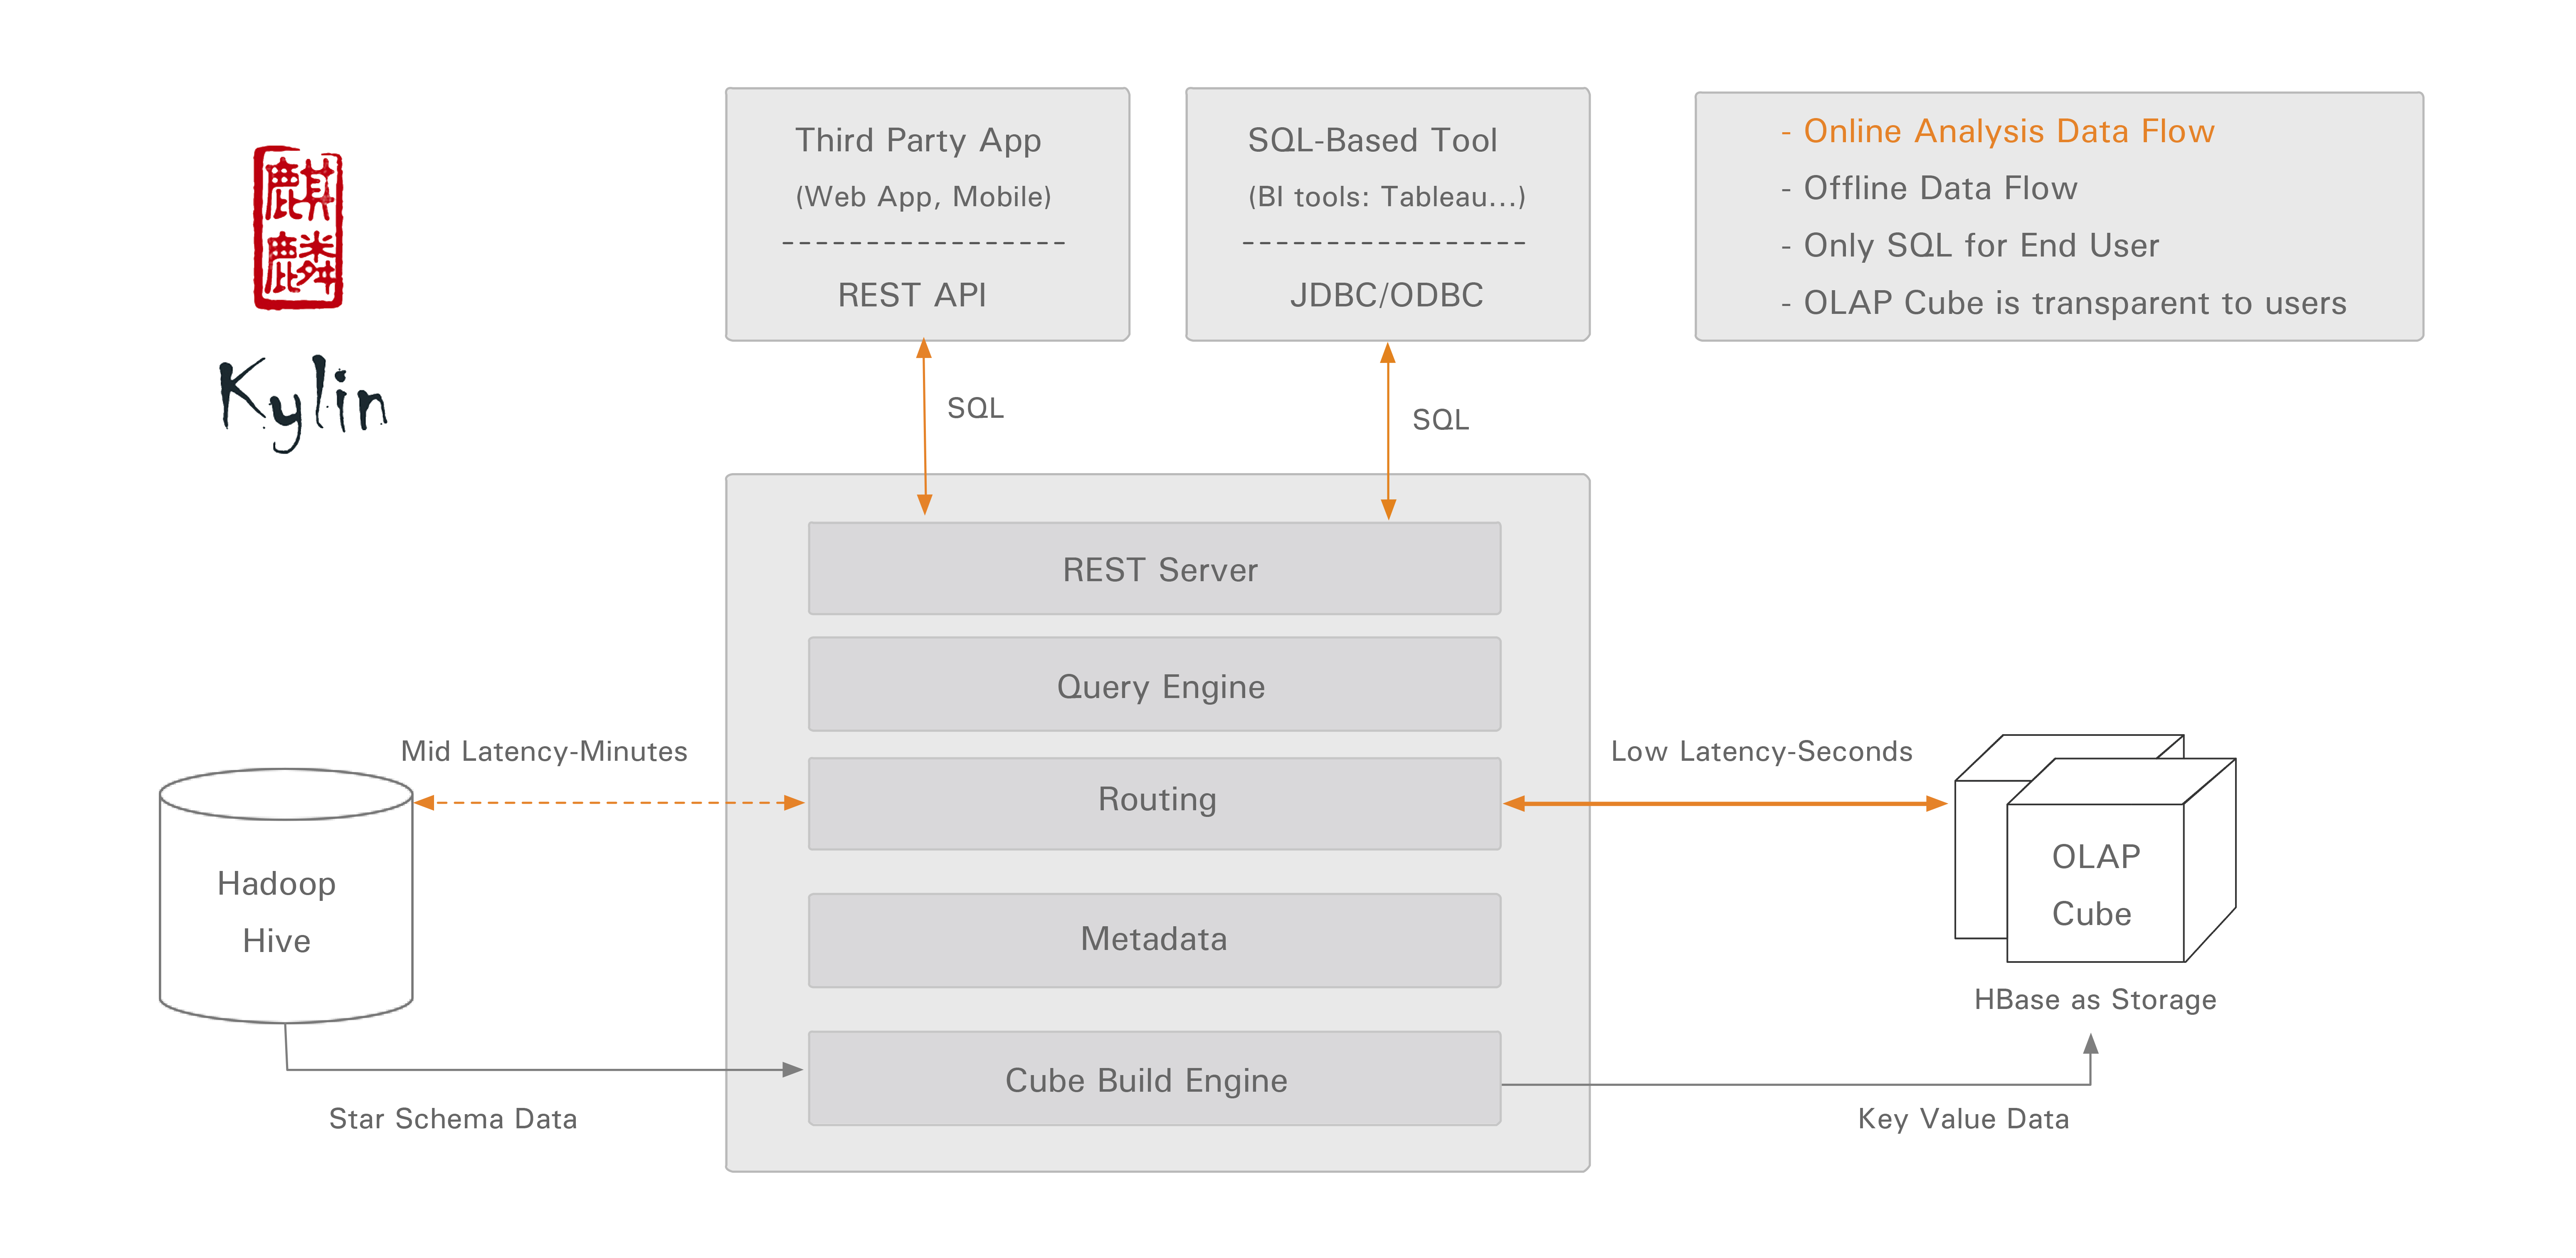
\includegraphics[width=10cm,height=8cm]{ppt_figures/kylin_diagram.png}
\end{frame}

\subsection{Data Mining}
\begin{frame}{Data Mining}
	\begin{itemize}
		\item John Naisbett (author of famous `Megatrends') said ``We are drowning in information but starved for knowledge''
		\item Data mining techniques can broadly be classified into two categories
		\begin{itemize}
			\item Supervised learning
			\item Un-Supervised learning
		\end{itemize}
	\end{itemize}
\end{frame}
\begin{frame}{Data Mining(contd.)}
	Supervised Learning : The dependent and control variables are known. Classification and regression algorithms
	\begin{itemize}
		\item Linear 
		\item Multiple 
		\item Nonlinear
		\item Logistic
		\item Decision tree
		\item Random forest
	\end{itemize}
	
\end{frame}
\begin{frame}{Data Mining(contd.)}
	Un-Supervised Learning : The dependent and independent variables are unknown
	\begin{itemize}
		\item k means clustering
		\item Apriori clustering
		\item Hierarchical clustering
		\item Hidden Markov models
		\item Self Organizing Maps
	\end{itemize}
\end{frame}

\begingroup
\small
\begin{frame}
	\frametitle{Choosing the Right Data Mining Technique}
	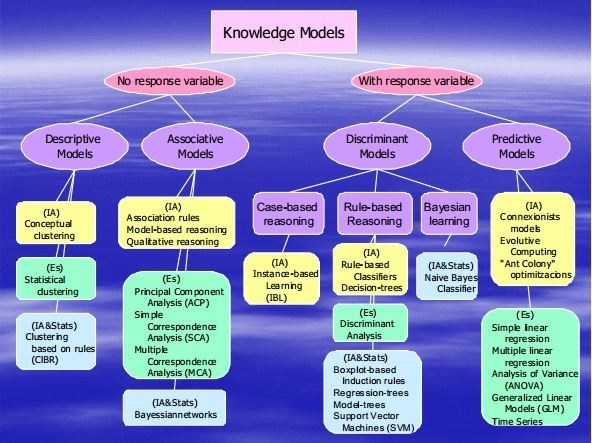
\includegraphics[width=\columnwidth,height=8cm]{ppt_figures/selectionofdatamining.jpeg}
\end{frame}

\begin{frame}{Scikit model selection}
	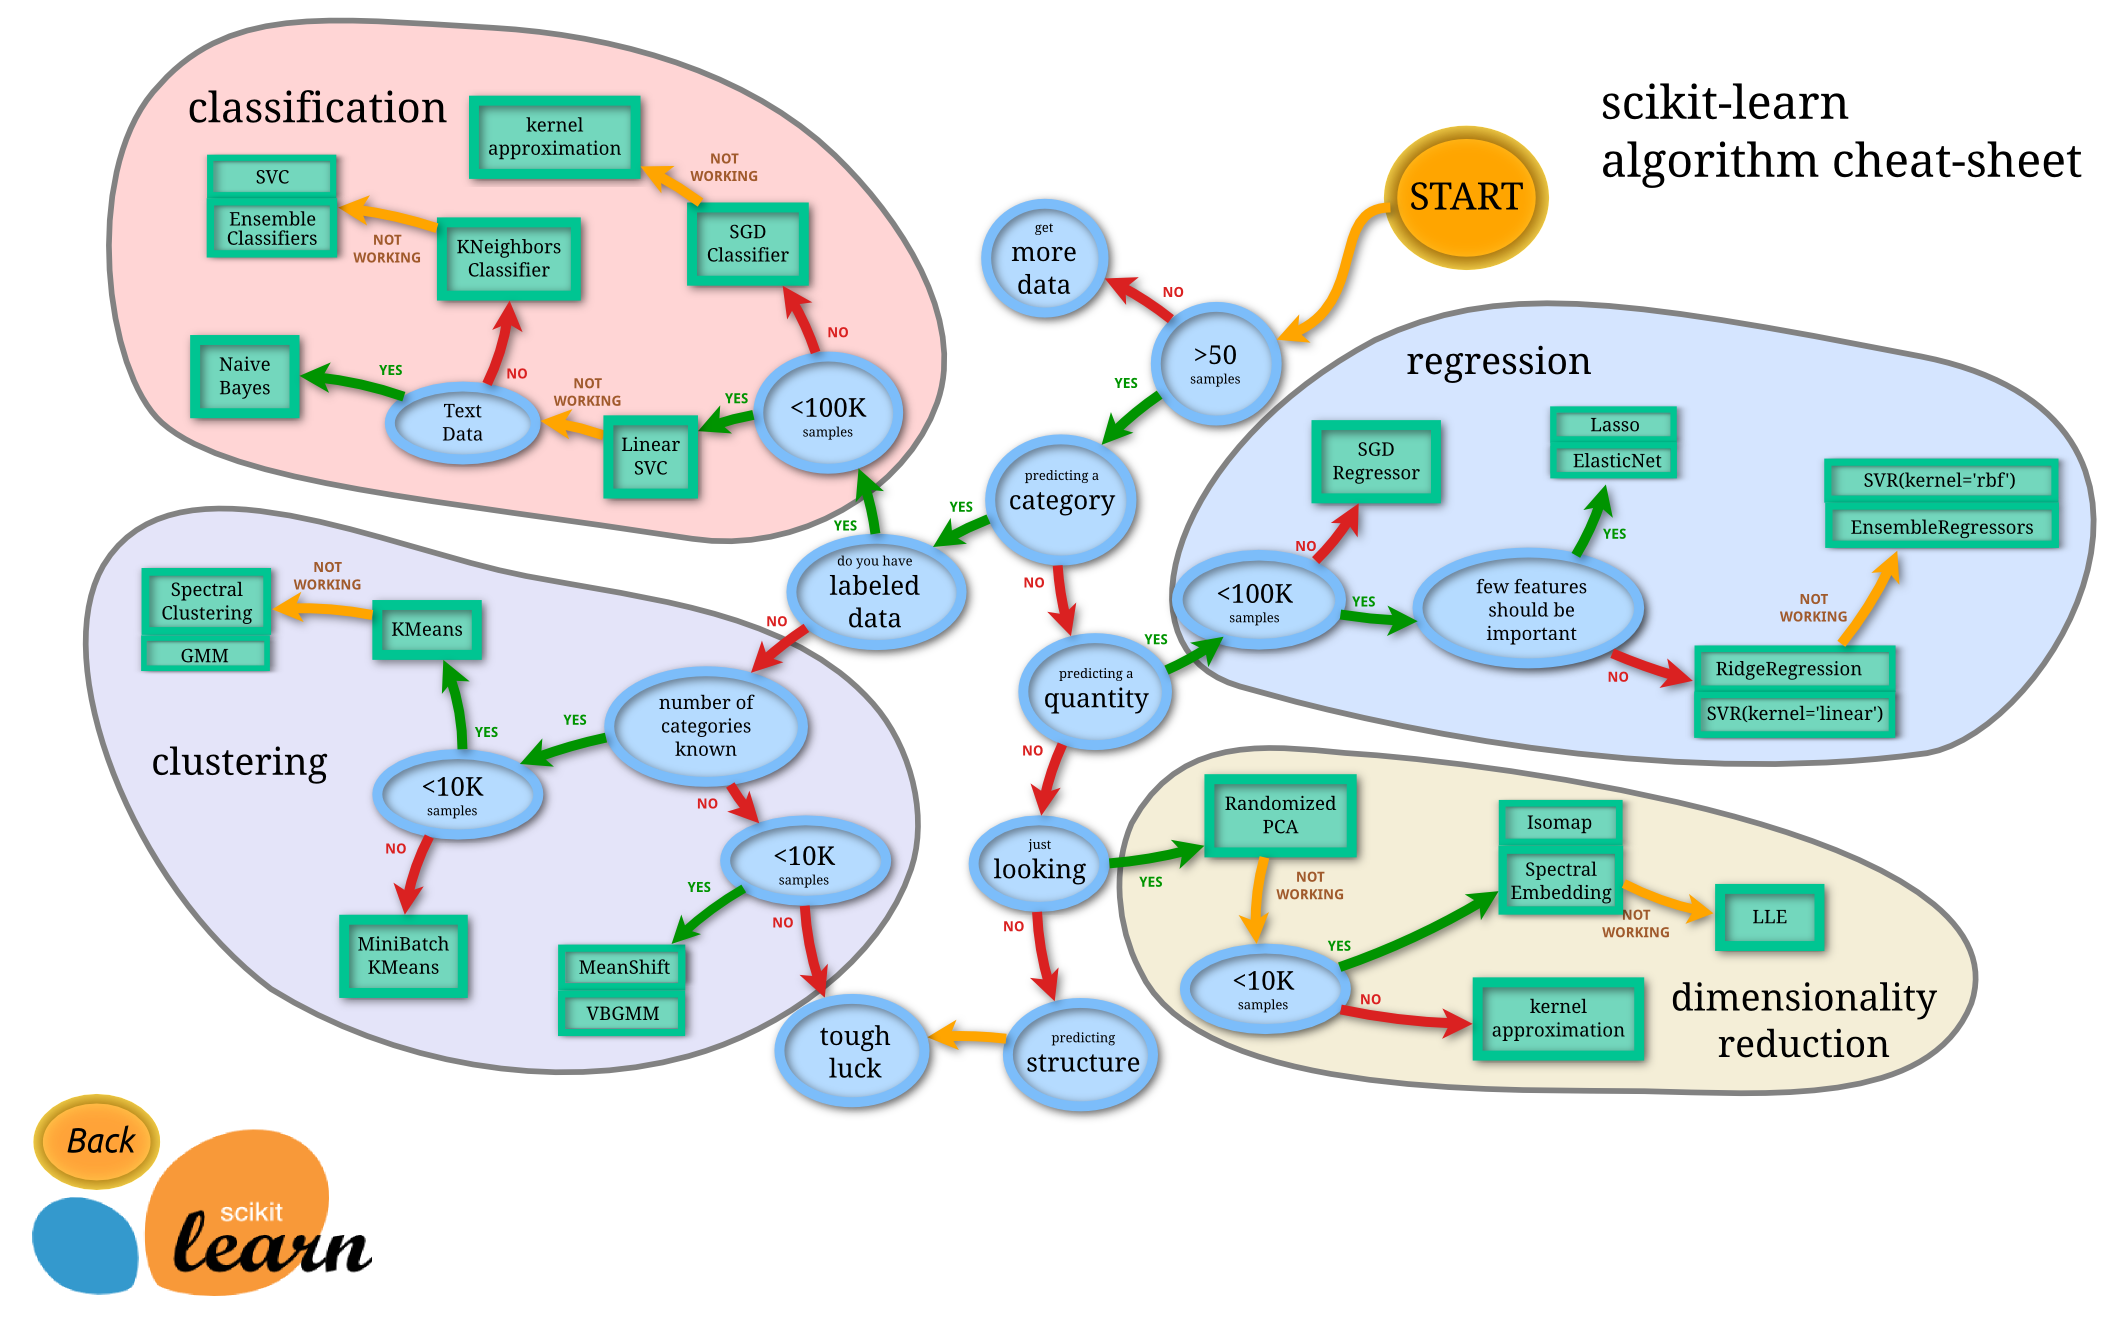
\includegraphics[width=\columnwidth,height=8cm]{ppt_figures/scikitlearn.png}
\end{frame}
\endgroup


\begin{frame}{Data Mining(contd.)}
	Softwares
		\begin{itemize}
			\item Weka
			\item Knime
			\item Rapidminer
		\end{itemize}
	Libraries
		\begin{itemize}
			\item Tensorflow
			\item mlpack
			\item H20
			\item Mlib
			\item Scikit
		\end{itemize}
	Servers 
		\begin{itemize}
			\item DeepDetect
			\item Apache PredictionIO
			\item Shiny
		\end{itemize}
\end{frame}

\begin{frame}{Apache PredictionIO}
	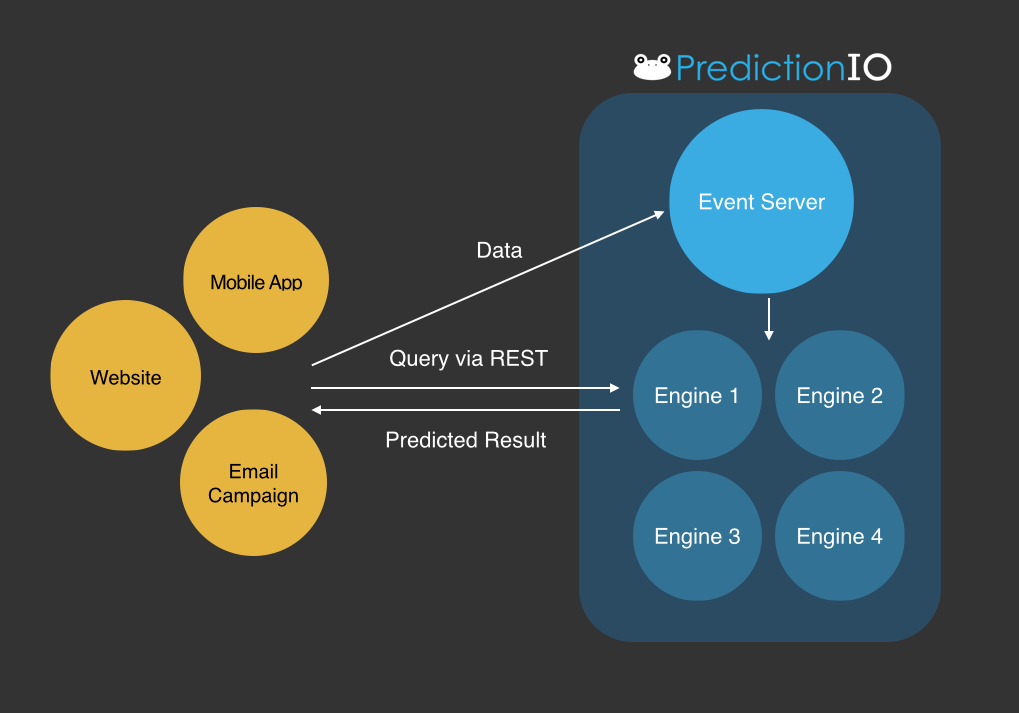
\includegraphics[width=\textwidth,height=8cm]{ppt_figures/predictionioeventsever.png}
\end{frame}

\begin{frame}{Shiny Architecture}
	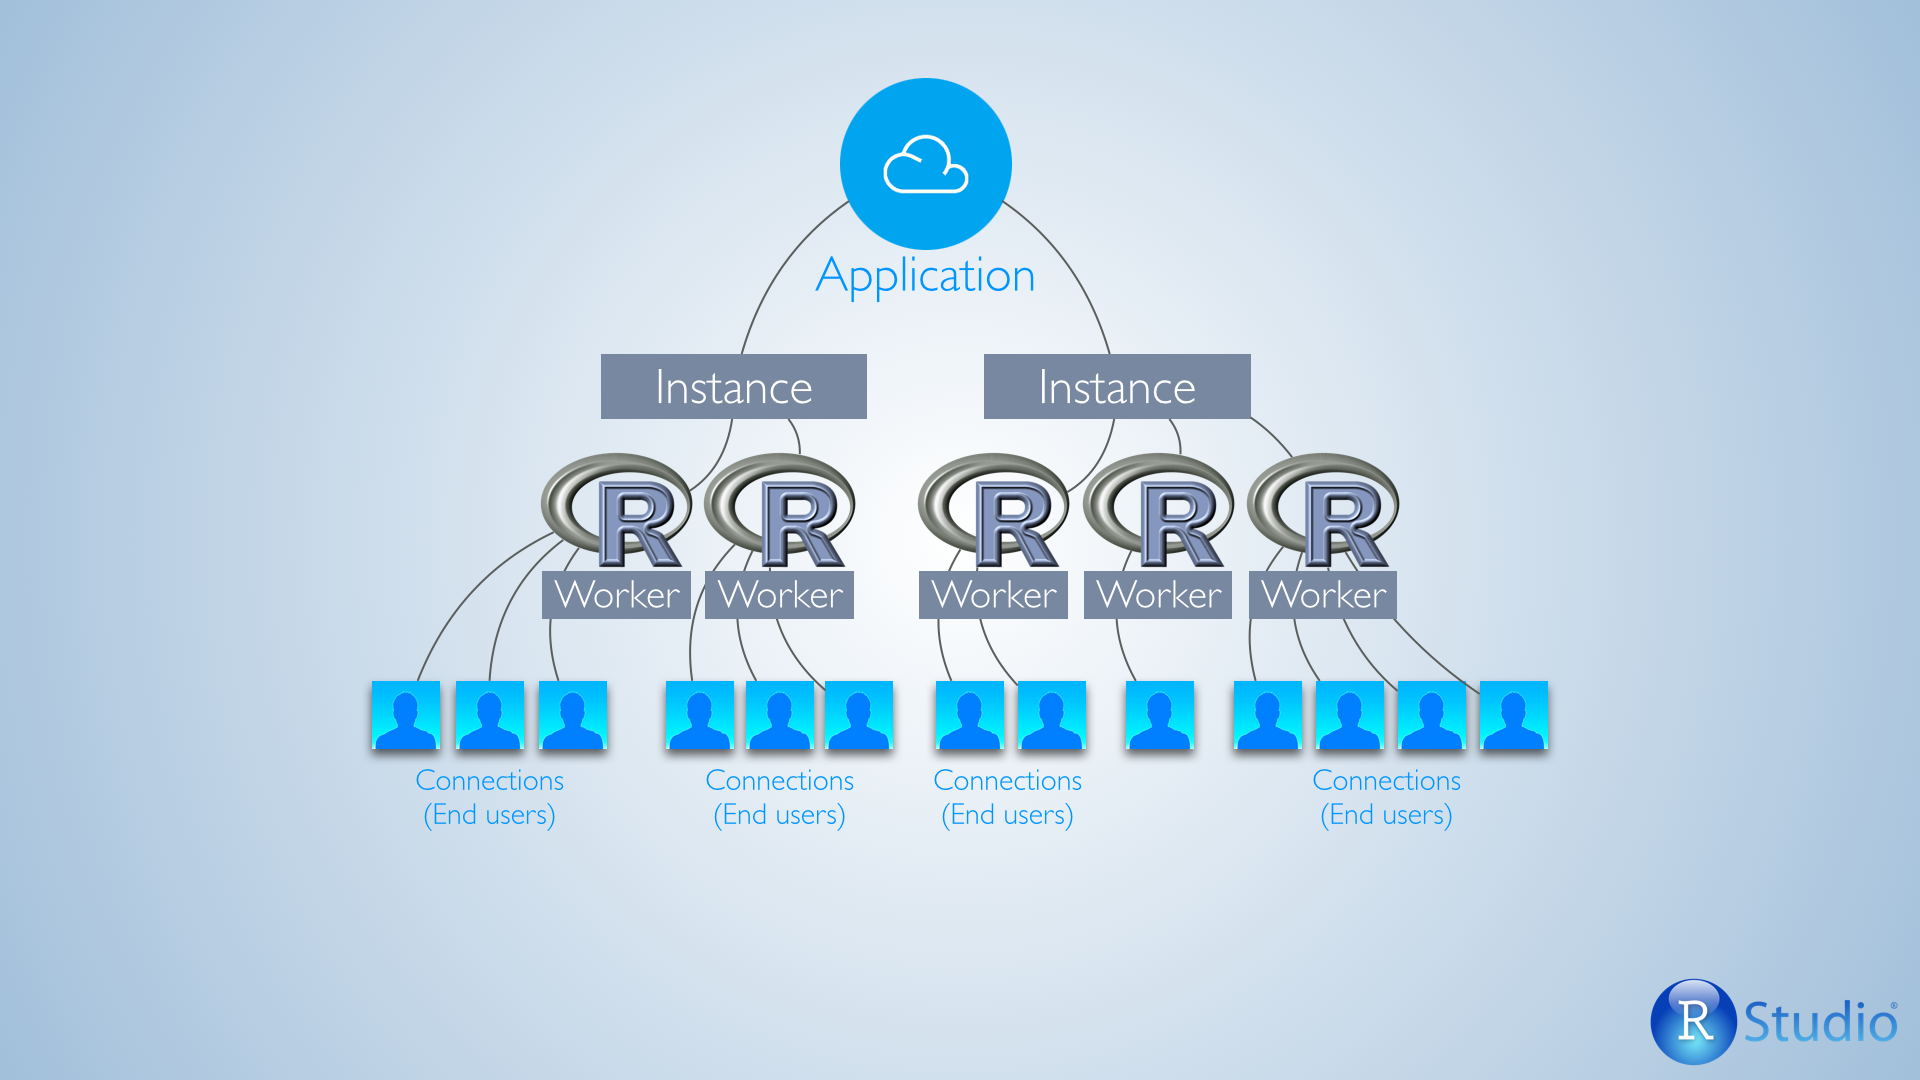
\includegraphics[width=\textwidth,height=8cm]{ppt_figures/shinyscaling.png}
	\end{frame}
	
	
\subsection{Model Evaluation Metrics}
\begin{frame}{Model Evaluation Metrics}
	\begin{itemize}
		\item Holdout technique
		\item k-fold Cross validation technique
		\item Sentivity and Specificity
	\end{itemize}
\end{frame}

\subsection{Review of Selected Research Papers}
\begin{frame}{Review of Selected Research Papers}
	Present 3 papers which are relevant to Churn prediction
	\begin{itemize}
		\item Modeling \& Simulation of a Predictive Customer Churn Model for Telecommunication Industry
		\item A Hybrid Churn Prediction Model in Mobile Telecommunication Industry
		\item A comparison of machine learning techniques for customer churn prediction
	\end{itemize}
\end{frame}

\begin{frame}{Review of Selected Research Papers(contd.)}
	Modeling \& Simulation of a Predictive Customer Churn Model for Telecommunication Industry
	\begin{itemize}
		\item Technique used by researchers was a Fuzzy inference system
		\item Combination of Neural network with fuzzy logic
		\item They modeled Membership functions for the attributes
		\item Data used was call detail record of 5000 subscribers 
		\item It has 21 attributes and only 9 were selected
		\item Precision around 80\%; Recall of 92.7\% and Accuracy 95.8\%
	\end{itemize}
\end{frame}

\begin{frame}{Review of Selected Research Papers(contd.)}
	A Hybrid Churn Prediction Model in Mobile Telecommunication Industry
	\begin{itemize}
		\item Presents a combination of Voted Perceptron and Logistic regression
		\item Compared performance with Logistic regression and Voted perceptron as individual prediction models
		\item WEKA software was used to model the predictors
		\item Call detail records of 2000 customers was sourced from Asian telecom company
		\item 23 attributes were used for modeling
		\item Results : Hybrid models performed better than individual models
	\end{itemize}
\end{frame}

\begin{frame}{Review of Selected Research Papers(contd.)}
	A comparison of machine learning techniques for customer churn prediction
	\begin{itemize}
		\item researchers present a well meted out comparison between the normal model functions
		and their corresponding boosted models
		\item performance criteria was based on the F-score
		\item series of simulations based on the Monte Carlo method
		\item 5 DM techniques - Back-Propagation algorithm , Support Vector Machines, Decision Trees, Naive Bayes and
		Logistic Regression.
		\item churn dataset hosted at UCI Machine learning repository
		\item 100-fold cross validation technique was used to reduce bias
		\item Ratio of training to testing set is about $2 : 3$
	\end{itemize}
\end{frame}

\begin{frame}{Review of Selected Research Papers(contd.)}
	\begin{itemize}
		\item boosting algorithm Adaboost Adaboost.M1
		\item R programming was used for modeling the simulation experiment
		\begin{enumerate}
			\item tested classifiers run with data and performance of F-score measured
			\item boosting algorithm was applied and performance F-score measured
		\end{enumerate}
		\item Results
		\begin{itemize}
			\item Best performance : 2 layer BPN with 15 hidden nodes and Decision tree classifier
			\item SVM scored lower followed by Naive Bayes and Logit Regression at last.
			\item After boosting SVM got best performance accuracy of 97\% and F-score 84\%
		\end{itemize}
	\end{itemize}
\end{frame}

%------------------------------------------------Section
\section{Methodology}

\subsection{Research Methodology}
\begin{frame}{Research Methodology}
	\begin{figure}
		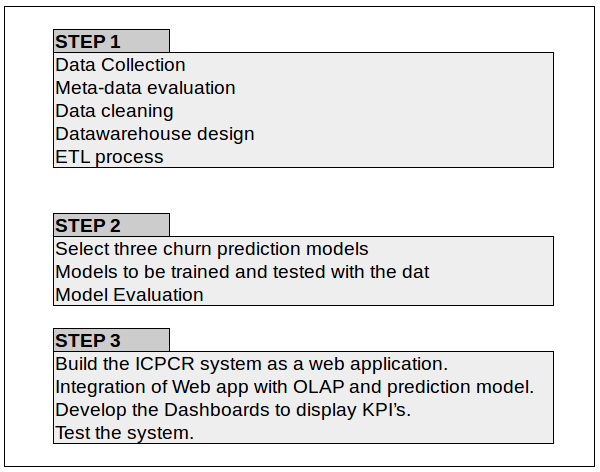
\includegraphics[scale = 0.35]{ppt_figures/ICPCR.png}
		\centering
		\caption{Research Methodology}
	\end{figure}
%	\begin{itemize}
%		\item {
%			3 steps to be implemented.
%		}
%		\item {
%			My second point.
%		}
%	\end{itemize}
\end{frame}

\subsection{Data Preprocessing and Datawarehouse Development }
\begin{frame}{Data Preprocessing and Datawarehouse Development}
	\begin{figure}[h]
		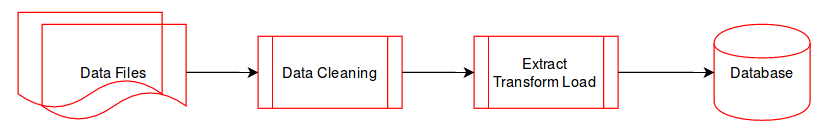
\includegraphics[scale = 0.35]{ppt_figures/dataloadprocess.png}
		\centering
		\caption{Data preprocessing}
	\end{figure}
	 \begin{figure}
	 	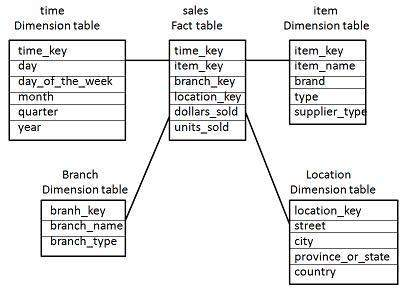
\includegraphics[scale = 0.35]{ppt_figures/olap_start_schema.jpg}
	 	\centering
	 	\caption{OLAP Star Schema}
	 \end{figure}
\end{frame}

\subsection{Development and Evaluation of the Prediction Models}
\begin{frame}{Development and Evaluation of the Prediction Models}
	\begin{itemize}
		\item Model design
		\begin{itemize}
			\item Proposal is to model 3 techniques based on Decision Tree, SVM, ANN
			\item To use Machine learning libraries of either MLib, Scikit or R
			\item Propose to implement a boosting algorithm Adaboost			
		\end{itemize}
		\item Model evaluation
		\begin{itemize}
			\item K-fold cross validation technique
			\item Confusion matrix with scoring of Sensitivity, Specificity, Precision and Recall, F-score 
		\end{itemize}
	\end{itemize}
\end{frame}

\subsection{System Development \& Evaluation}
\begin{frame}{System Development \& Evaluation}
	\begin{columns}
		\column{0.5\textwidth}
			4 steps to be implemented.
	\begin{itemize}
		\item Presentation Layer
		\begin{itemize}
			\item GUI for KPI's
			\item Plots of predictions
		\end{itemize}
		\item Application Layer
		\begin{itemize}
			\item Application processing
			\item Predictive model
			\item OLAP cube
		\end{itemize}
		\item Database Layer
		\begin{itemize}
			\item Data warehouse tables in star schema
			\item Data from prediction
		\end{itemize}
		\item System Testing 
		\begin{itemize}
			\item Unit testing and Latency tests
		\end{itemize}
	\end{itemize}
			\column{0.5\textwidth}
	\begin{figure}
		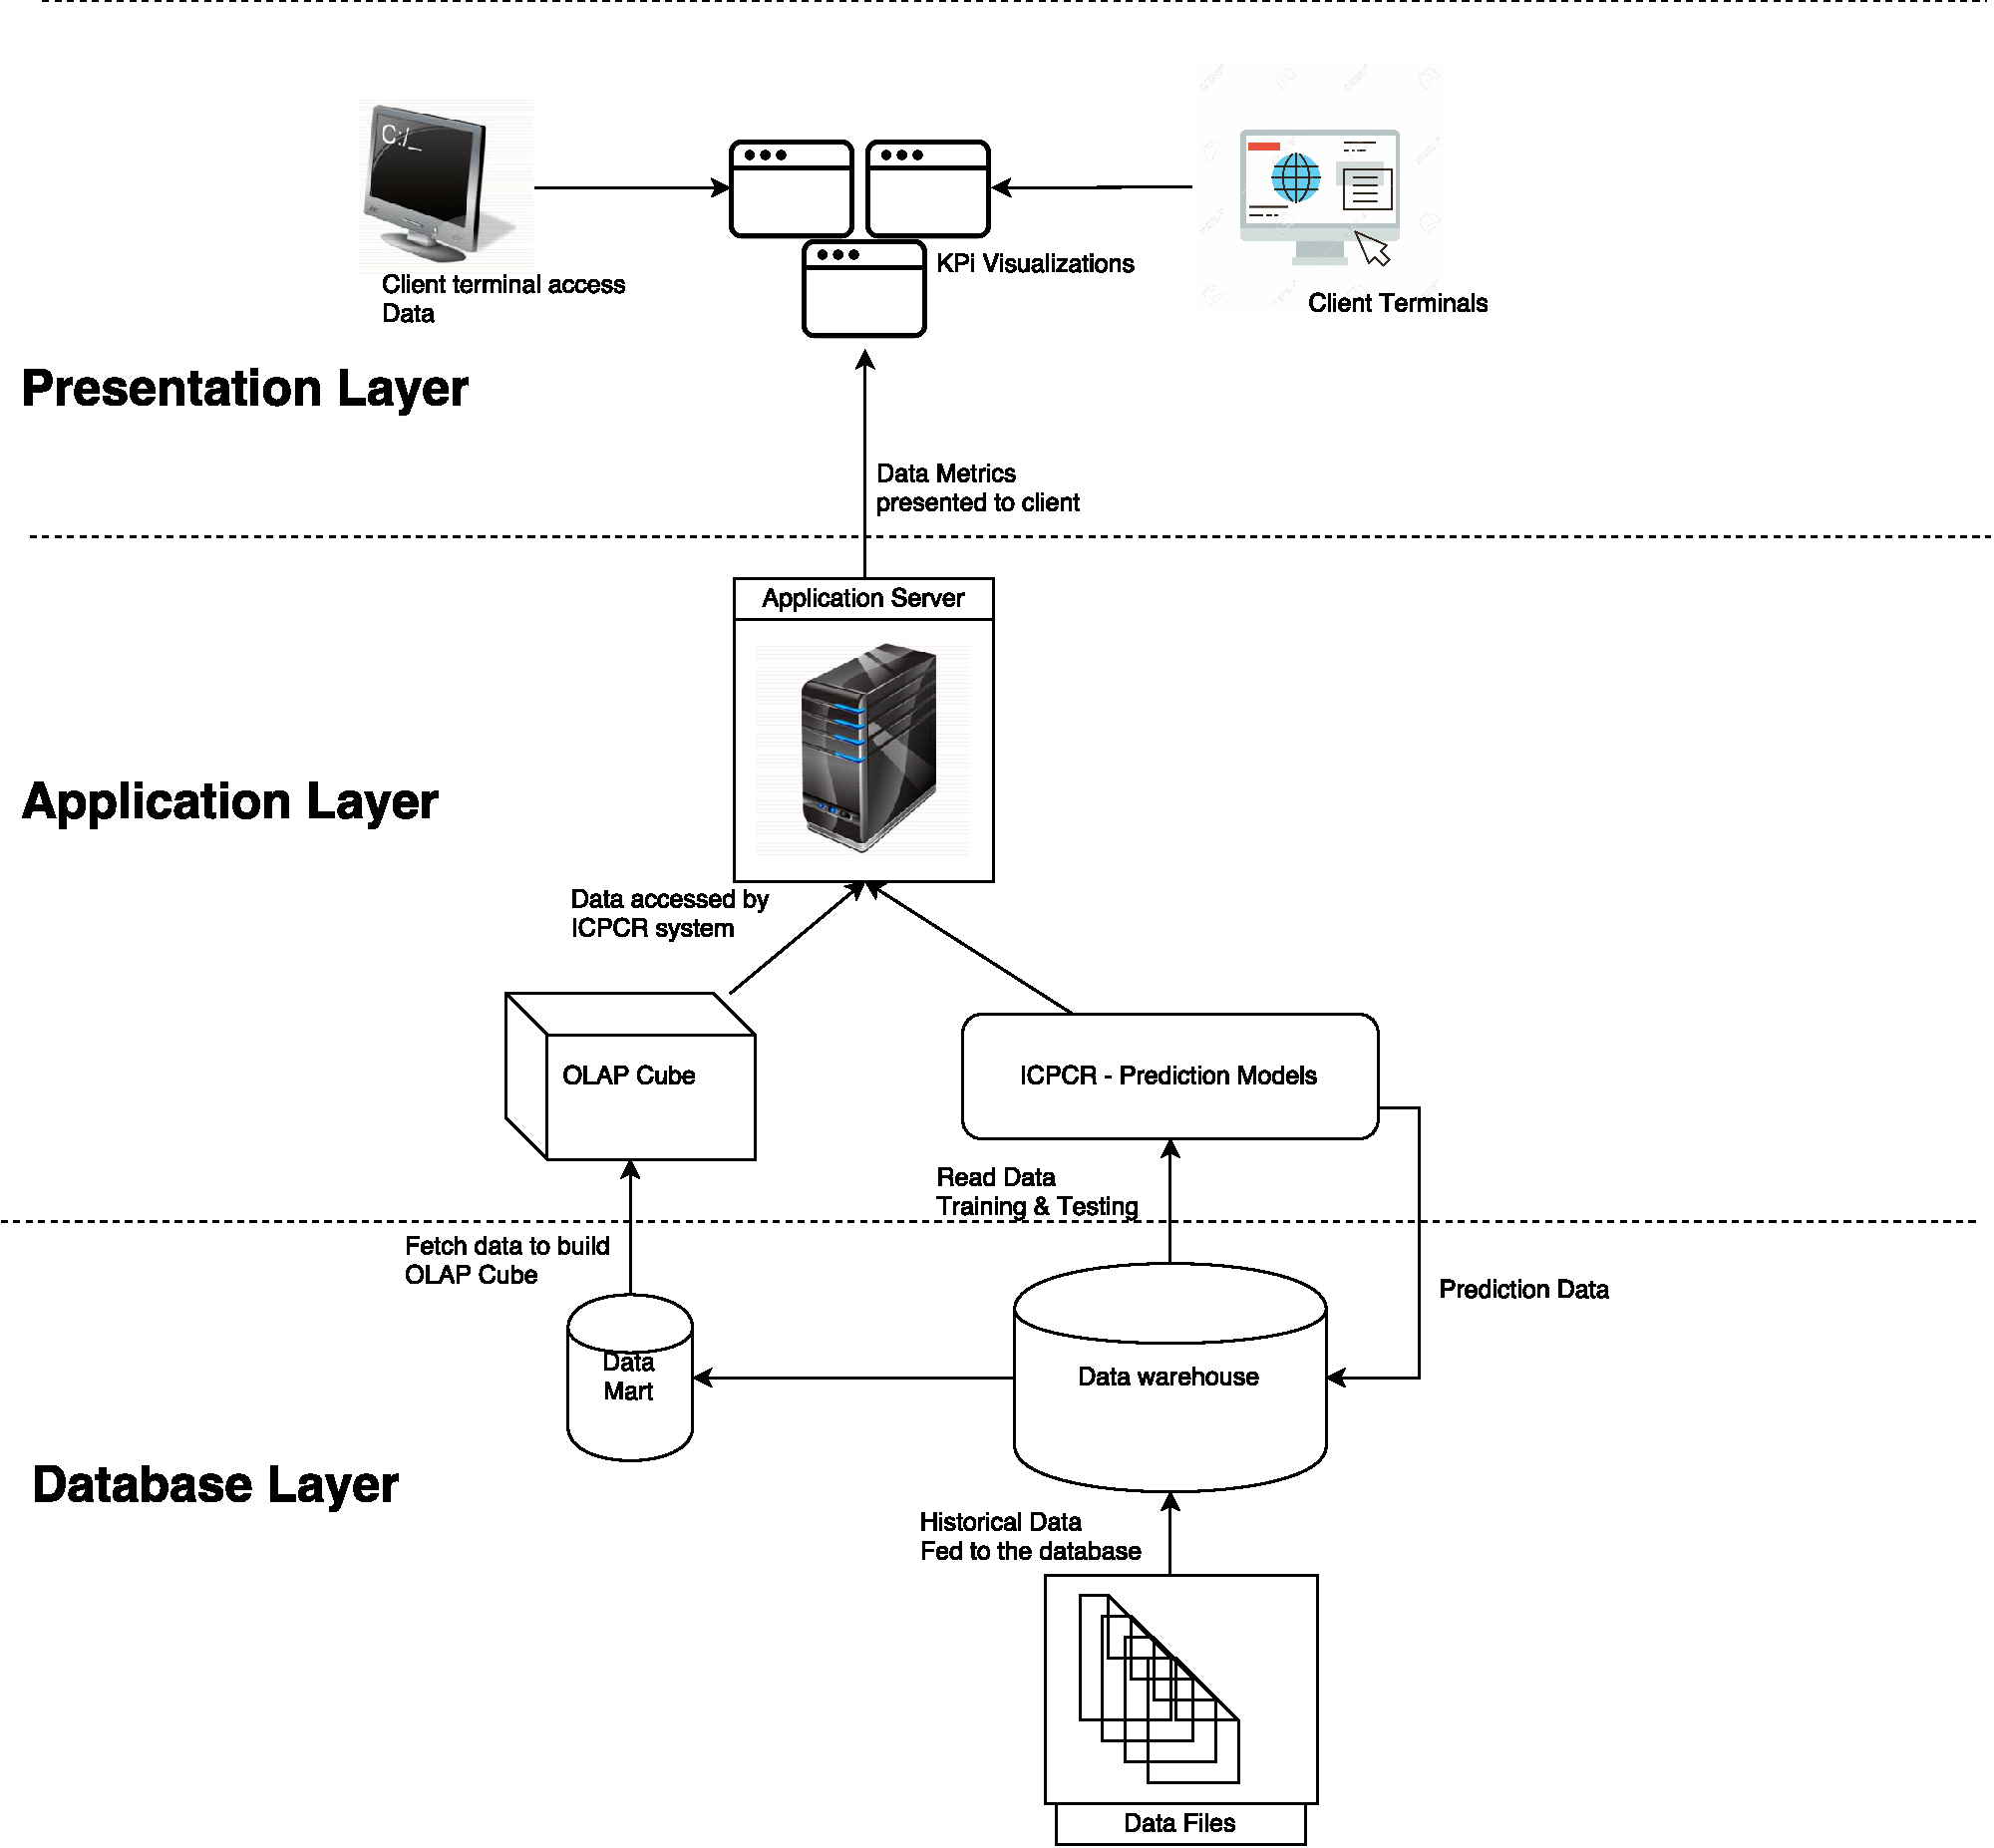
\includegraphics[width=7cm,height=7cm]{ppt_figures/ICPCR_pic1SystemDesign}
		\centering
	\end{figure}
		\end{columns}
\end{frame}

\begin{frame}{The Intelligent Churn Prediction Architecture}
	\begin{figure}[h]
		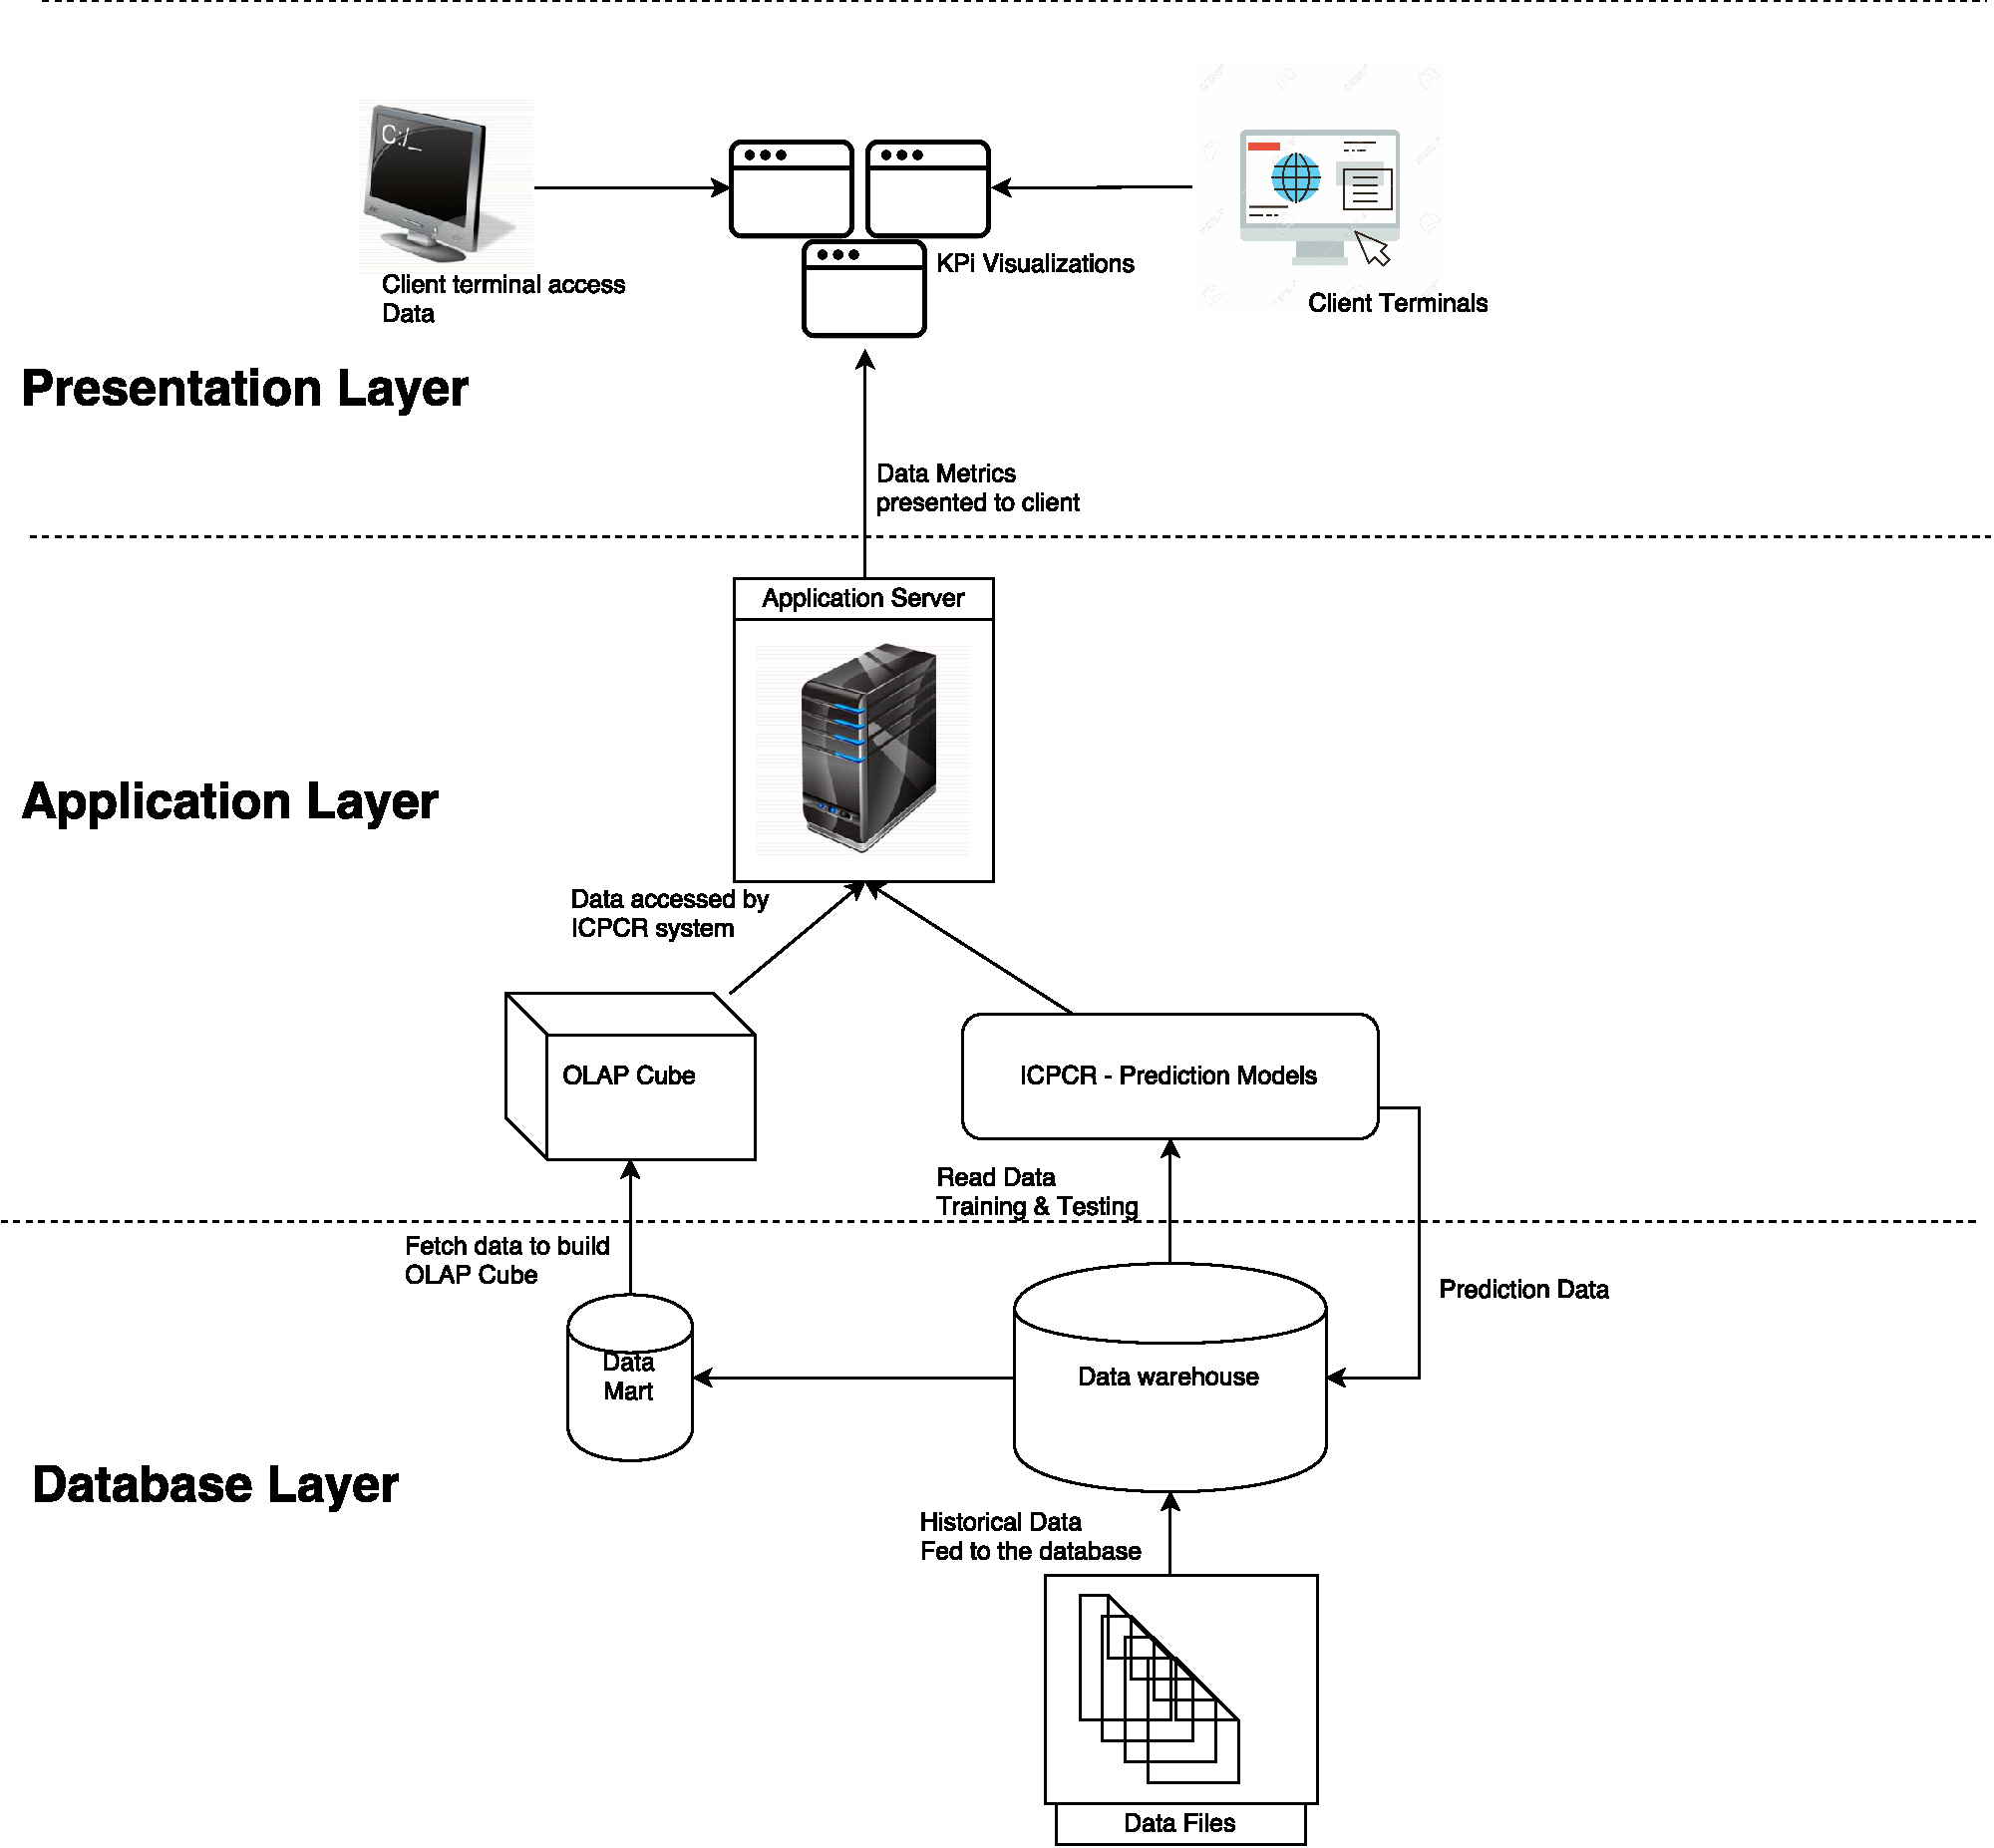
\includegraphics[width=9cm,height=7cm]{ppt_figures/ICPCR_pic1SystemDesign}
		\centering
	\end{figure}
\end{frame}

\subsection{Timeline}
\begin{frame}{Timeline}
\begin{figure}
	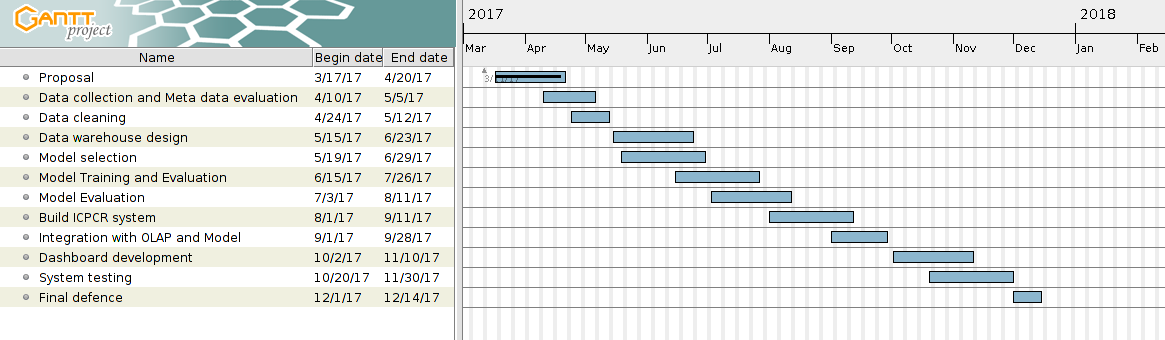
\includegraphics[width=13cm, height=8cm]{ppt_figures/churngantt3.png} 
%  	\centering
  \end{figure}
\end{frame}

%------------------------------------------------Section
\section{Progress}

\subsection{Data Collection}
\begin{frame}{Data Collection}
	\begin{itemize}
		\item Churn data taken from the SGI Machine learning repository
		\item Dataset has 21 Dimensions
		\item Data has 5000 records of data
	\end{itemize}	
\end{frame}
\begin{frame}{Meta-Data}
	\Fontmetadata
	\begin{table}[]
		\centering
		\caption{Variable descriptions}
		\label{var-1}
		\begin{tabular}{llll}
			\hline
			SNo & Name of Variable & Description            & Type                \\
			\hline
			1 & State            & state`s of USA           & discrete            \\
			2 & Account Length   & months of active usage & continuous  \\
			3 & Area code        & area code for phone  & continuous          \\
			4 & Phone number     & phone number  & discrete           \\
			5 & voice mail plan & Subscribed to voice mail & discrete   \\
			6 & number vmail messages & number of voice-mail messages &  continuous   \\
			7 & international plan & Subscribed to international plan &  discrete   \\
			8 & total intl minutes &  total number of international calls  &  continuous   \\
			9 & total intl calls & total charge of international calls &  continuous   \\
			10 & total intl charge & total charge of international calls                       &  continuous   \\
			\hline
		\end{tabular}

	\end{table}
\end{frame}
\begin{frame}{Meta-Data}
	\Fontmetadata

	\begin{table}[]

%		\centering
		\caption{Variable descriptions}
		\label{var-2}
		\hspace*{-0.5cm}		\begin{tabular}{llll}
			\hline
			SNo & Name of Variable & Description            & Type                \\
			\hline
			11 & total day minutes &  total minutes of day calls  &  continuous   \\
			12 & total day calls & total number of day calls &  continuous   \\
			13 & total day charge & total charge of day calls &  continuous   \\
			14 & total eve minutes & total minutes of evening calls &  continuous   \\
			15 & total eve calls & total number of evening call  &  continuous   \\
			16 & total eve charge & total charge of evening calls  &  continuous   \\
			17 & total night minutes & total minutes of night call &  continuous   \\
			18 & total night calls & total number of night calls &  continuous   \\
			19 & total night charge & total charge of night calls  &  continuous   \\
			20 & number customer service calls & number of calls to customer service &  continuous   \\
			21 & churn value & if customer churned or not & discrete \\
			\hline
		\end{tabular}
	\end{table}
\end{frame}
\begin{frame}{Data evaluation}
	Churn data statistics
	\begin{figure}
		\hspace*{-1cm}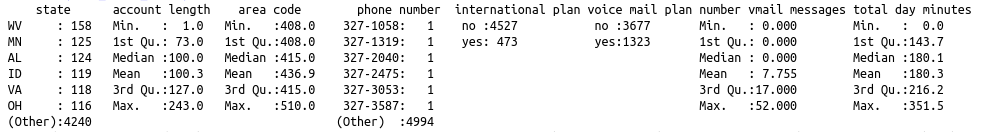
\includegraphics[width=13cm,height=2cm]{ppt_figures/data_summary_1}
%		\centering
	\end{figure}
	\begin{figure}
		\hspace*{-1cm}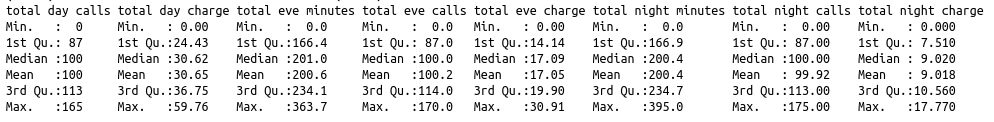
\includegraphics[width=13cm,height=2cm]{ppt_figures/data_summary_2}
	\end{figure}

\end{frame}

\begin{frame}{Data evaluation contd. }
	\begin{figure}
		\hspace*{-1cm}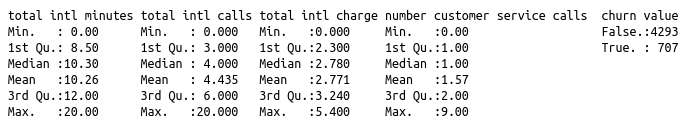
\includegraphics[width=13cm,height=2cm]{ppt_figures/data_summary_3}
	\end{figure}
\end{frame}

\subsection{Models}
\begin{frame}{Churn prediction models}
	\begin{itemize}
		\item Support Vector Machine trained Linear and Radial models
		\item Decision Tree trained and predicted with  classification type dt
		\item Neural networks : Currently still in processing phase. Error with input variable types
	\end{itemize}
\end{frame}
\begin{frame}{Decision Tree 1}
	\begin{figure}
		\hspace*{-1cm}
		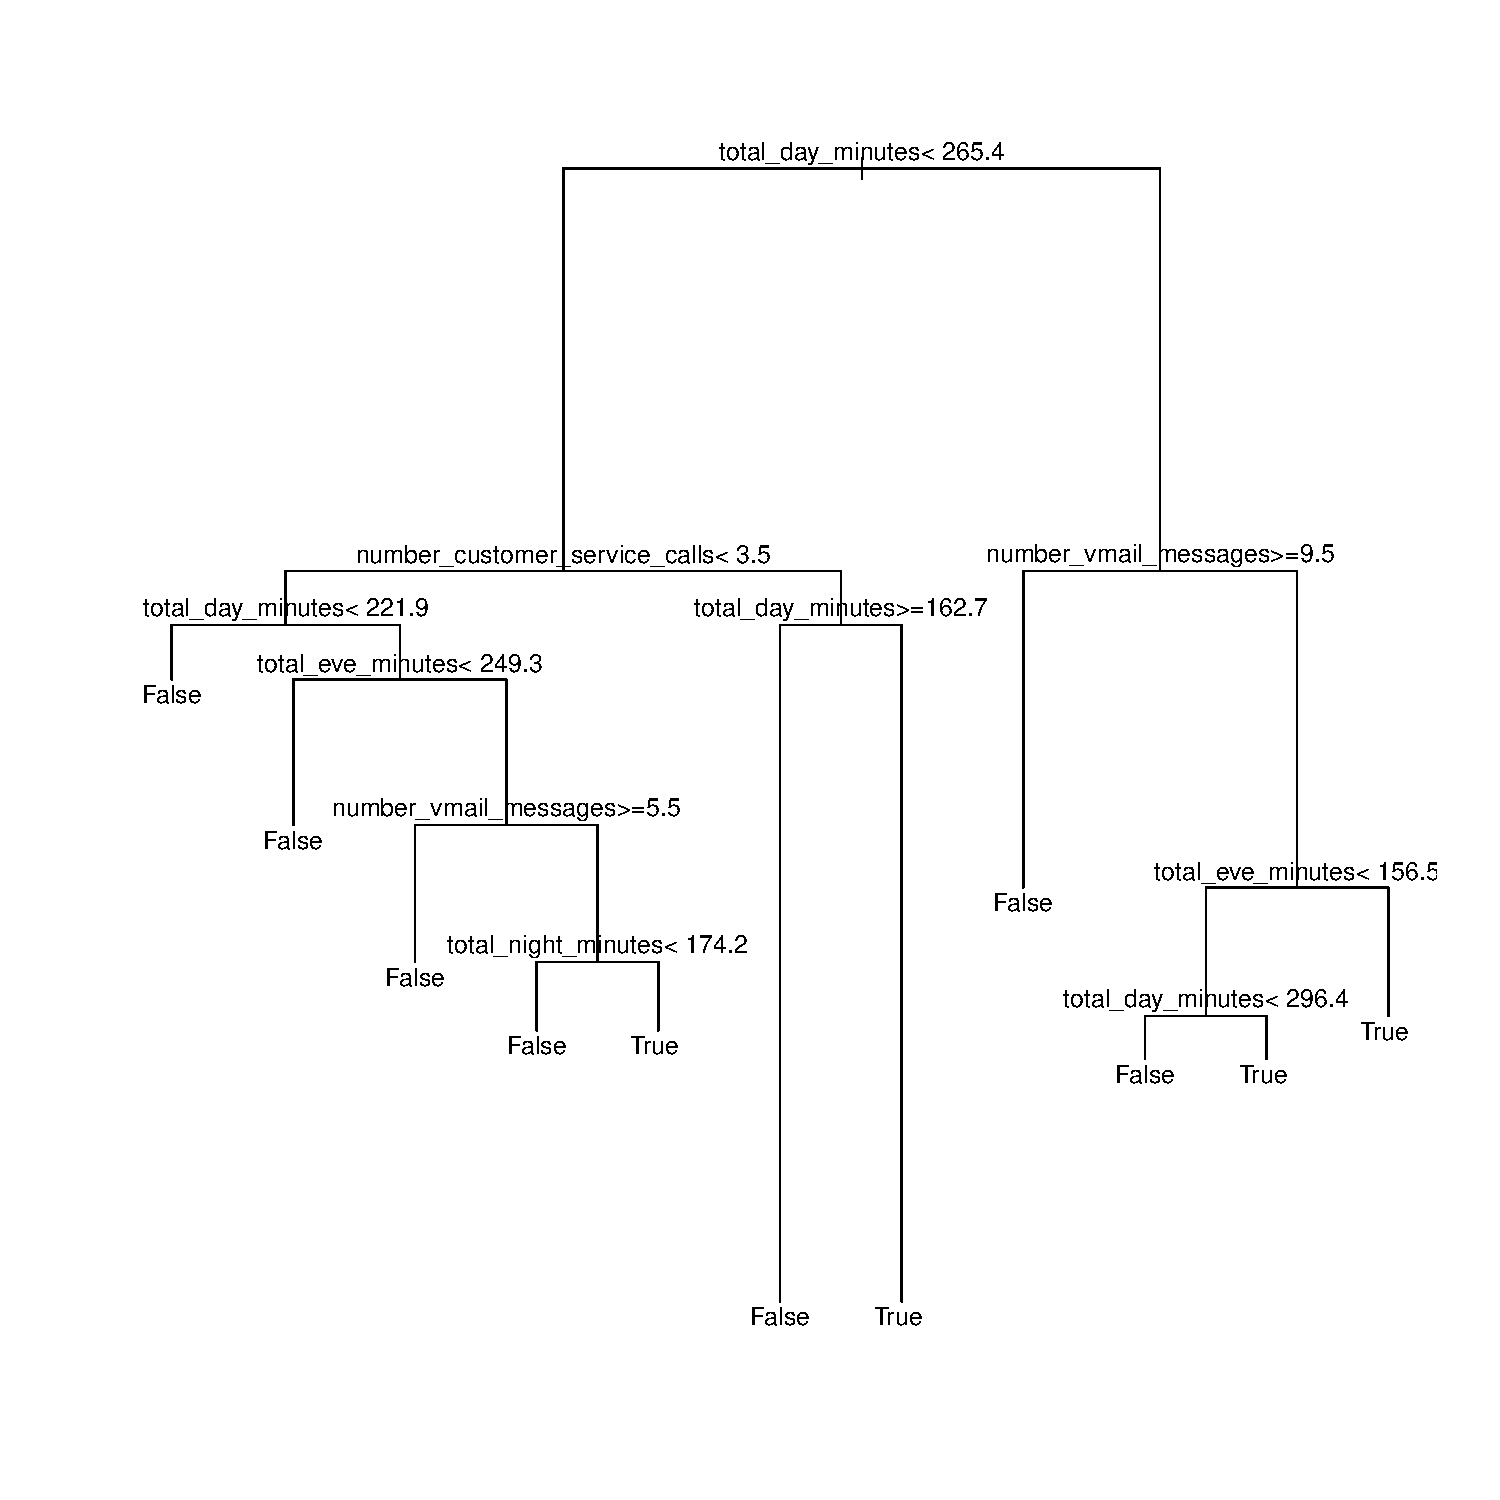
\includegraphics[width=13cm,height=10cm]{ppt_figures/churnDecisionTree}
	\end{figure}
\end{frame}

\begin{frame}{Decision Tree 1 Confusion Matrix}
	\begin{table}
		\begin{tabular}{lll}
						\hline
						Prediction & False & True \\
						\hline
						False & 1266 & 109 \\
						\hline
						True & 19 & 106 \\
						\hline
		\end{tabular}
	\end{table}
\end{frame}

\begin{frame}{Decision Tree 1 Statistics}
	\begin{table}[]
		\centering
		\caption{DT-1 Stats}
		\label{dt-1-stats}
		\begin{tabular}{p{5cm}p{1cm}p{5cm}}
			Accuracy  & : & 0.9146667 \\
			\hline
			95\% CI   & : & (0.8993698, 0.9283156) \\ \hline
			No Information Rate  & : & 0.8566667 \\ \hline
			P-Value {[}Acc \textgreater NIR{]}  & : & 0.00000000000511805609 \\ \hline
			Sensitivity  & : & 0.9852140 \\ \hline
			Specificity  & : & 0.4930233 \\ \hline
			
		\end{tabular}
	\end{table}
\end{frame}
\begin{frame}{Decision Tree 2}
	\begin{figure}
		\hspace*{-1cm}
		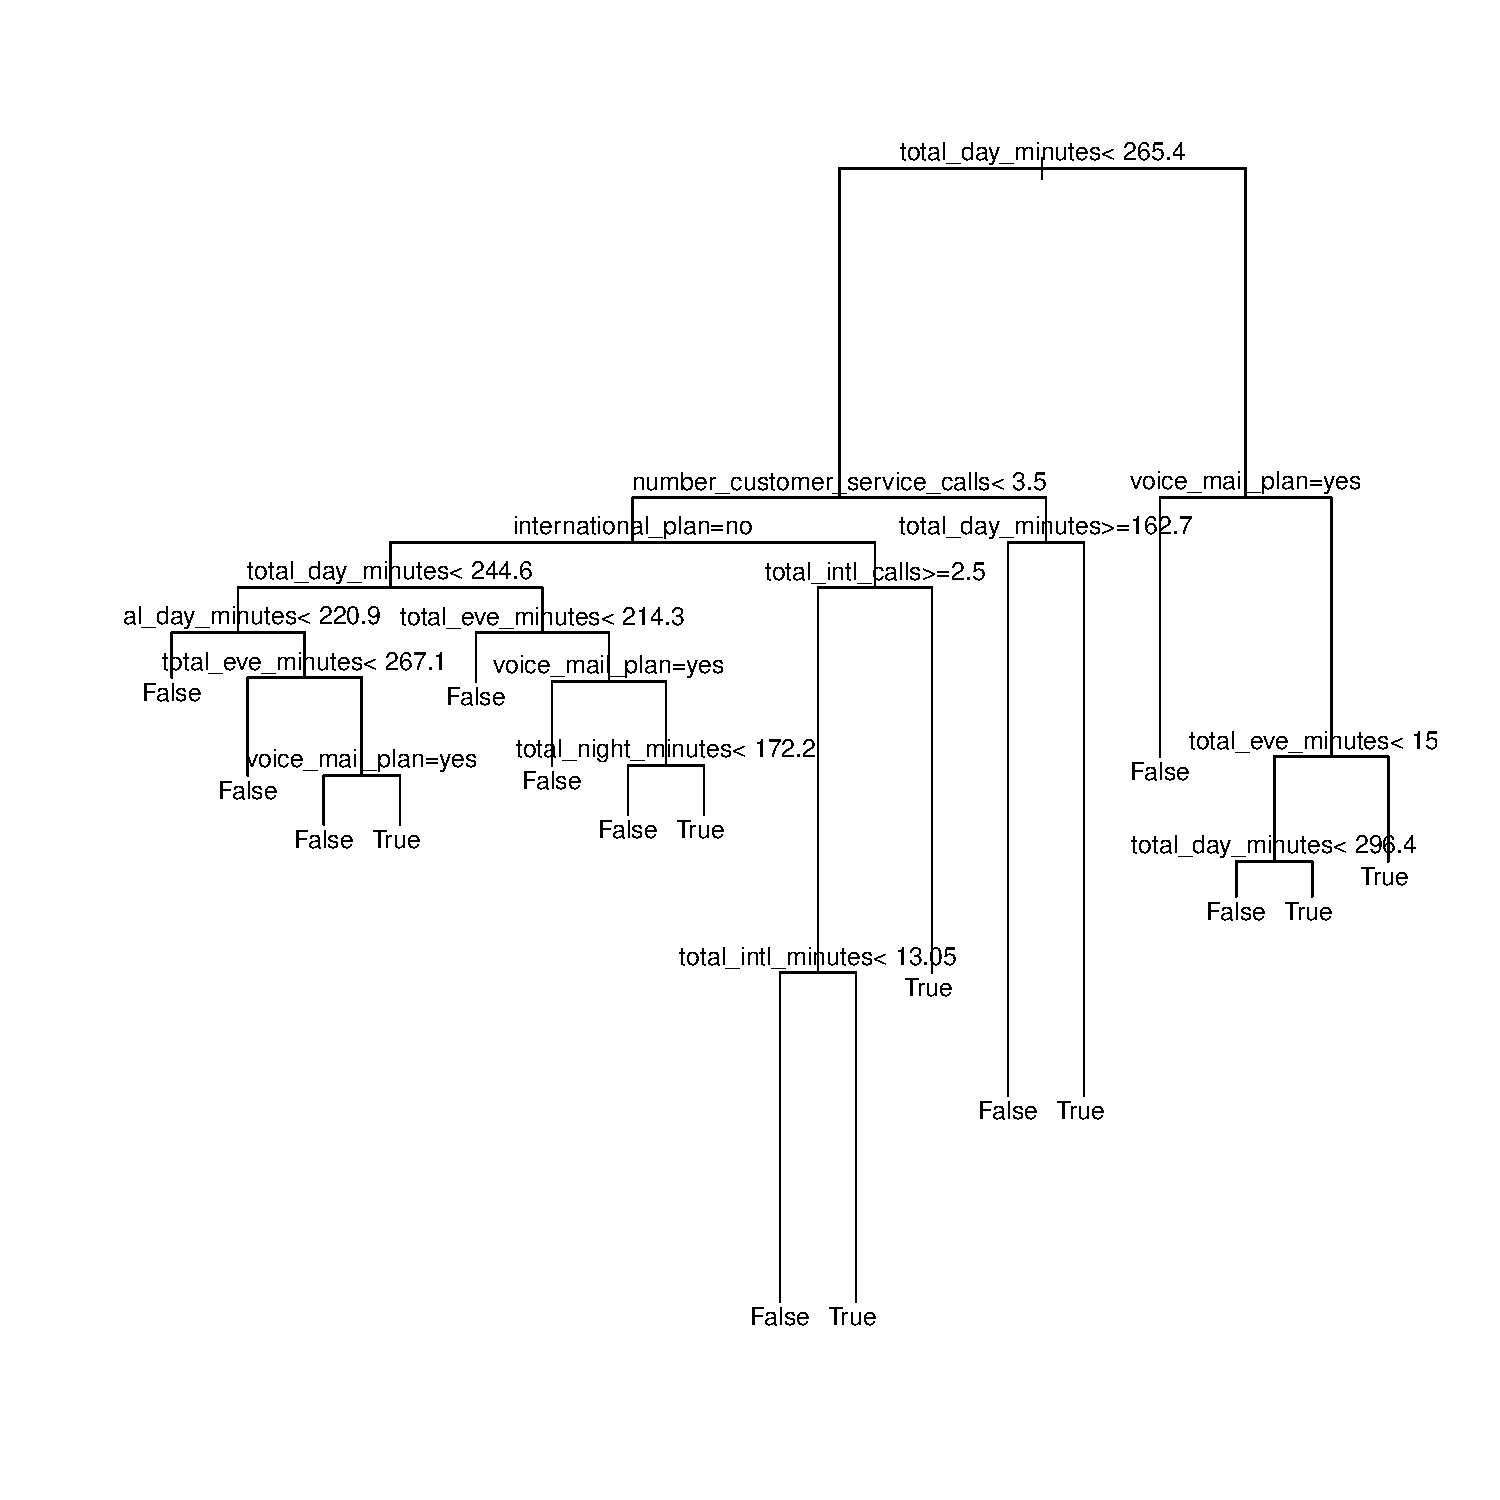
\includegraphics[width=13cm,height=10cm]{ppt_figures/churnDecisionTree1}
	\end{figure}
\end{frame}


\begin{frame}{Decision Tree 2 Confusion Matrix}
	\begin{table}
		\begin{tabular}{lll}
			\hline
			Prediction & False & True \\
			\hline
			False & 1266 & 68 \\
			\hline
			True & 19 & 147 \\
			\hline
		\end{tabular}
	\end{table}
\end{frame}

\begin{frame}{Decision Tree 2 Statistics}
	\begin{table}[]
		\centering
		\caption{DT-1 Stats}
		\label{dt-1-stats}
		\begin{tabular}{p{5cm}p{1cm}p{5cm}}
			Accuracy  & : & 0.942 \\
			\hline
			95\% CI   & : & (0.9289464, 0.9532869) \\ \hline
			No Information Rate  & : & 0.8566667 \\ \hline
			P-Value {[}Acc \textgreater NIR{]}  & : & 0.00000000000511805609 \\ \hline
			Sensitivity  & : & 0.9852140 \\ \hline
			Specificity  & : & 0.4930233 \\ \hline
			
		\end{tabular}
	\end{table}
\end{frame}

\begin{frame}{SVM Linear Kernel Stats}
	\begin{itemize}
		\item Training sameple : 	3500
		\item Testing sample : 1500
		\item 18 predictors
		\item 2 classes: 'False', 'True' 
		\item Pre-processing: centered (69), scaled (69) 
		\item Resampling: Cross-Validated (10 fold, repeated 3 times) 
%		\item Summary of sample sizes: 3150, 3151, 3150, 3150, 3150, 3149, ... 
		\item Resampling results
		\begin{itemize}
			\item Accuracy  0.8595245
			\item Kappa      0.003825618 
		\end{itemize}
	\end{itemize}
\end{frame}

\begin{frame}{SVM Linear Kernel Confusion Matrix}
	\begin{table}
		\begin{tabular}{lll}
			\hline
			Prediction & False & True \\
			\hline
			False & 1285 & 215 \\
			\hline
			True & 0 & 0 \\
			\hline
		\end{tabular}
	\end{table}
\end{frame}

\begin{frame}{SVM Linear Kernel Statistics}
	\begin{table}[]
		\centering
		\caption{SVM Linear Stats}
		\label{svm-l-stats}
		\begin{tabular}{p{5cm}p{1cm}p{5cm}}
			Accuracy  & : & 0.8567 \\
			\hline
			95\% CI   & : & (0.8379, 0.874) \\ \hline
			No Information Rate  & : & 0.8567 \\ \hline
			P-Value {[}Acc \textgreater NIR{]}  & : & 0.5182 \\ \hline
			Sensitivity  & : & 1 \\ \hline
			Specificity  & : & 0 \\ \hline
			
		\end{tabular}
	\end{table}
\end{frame}

\begin{frame}{SVM Radial Kernel Stats}
	\begin{itemize}
		\item Training sameple : 	3500
		\item Testing sample : 1500
		\item 18 predictors
		\item 2 classes: 'False', 'True' 
		\item Pre-processing: centered (69), scaled (69) 
		\item Resampling: Cross-Validated (10 fold, repeated 3 times) 
		%		\item Summary of sample sizes: 3150, 3151, 3150, 3150, 3150, 3149, ... 
		\item Resampling results
		\begin{itemize}
			\item Accuracy  0.8594297
			\item Kappa      0
		\end{itemize}
	\end{itemize}
\end{frame}

\begin{frame}{SVM Radial Kernel Confusion Matrix}
	\begin{table}
		\begin{tabular}{lll}
			\hline
			Prediction & False & True \\
			\hline
			False & 1266 & 68 \\
			\hline
			True & 19 & 147 \\
			\hline
		\end{tabular}
	\end{table}
\end{frame}

\begin{frame}{SVM Radial Kernel Statistics}
	\begin{table}[]
		\centering
		\caption{SVM Radial Stats}
		\label{dt-1-stats}
		\begin{tabular}{p{5cm}p{1cm}p{5cm}}
			Accuracy  & : & 0.8566667 \\
			\hline
			95\% CI   & : & (0.8379028, 0.8740215) \\ \hline
			No Information Rate  & : & 0.8566667  \\ \hline
			P-Value {[}Acc \textgreater NIR{]}  & : &  0.5181819 \\ \hline
			Sensitivity  & : & 1 \\ \hline
			Specificity  & : & 0 \\ \hline
			
		\end{tabular}
	\end{table}
\end{frame}
% system
\subsection{Dashboard of ICPCR}
\begin{frame}{ICPCR}
	It is a web application.
	Developed thus far is ui.r and server.r files .
	\begin{figure}
		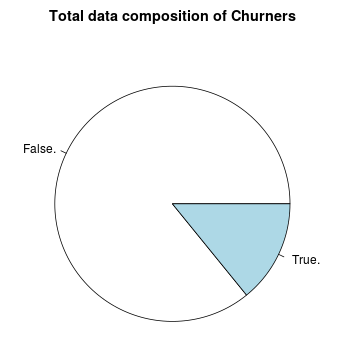
\includegraphics[scale=0.5]{ppt_figures/web_dash_1}
	\end{figure}
\end{frame}

\begin{frame}
	\begin{figure}
		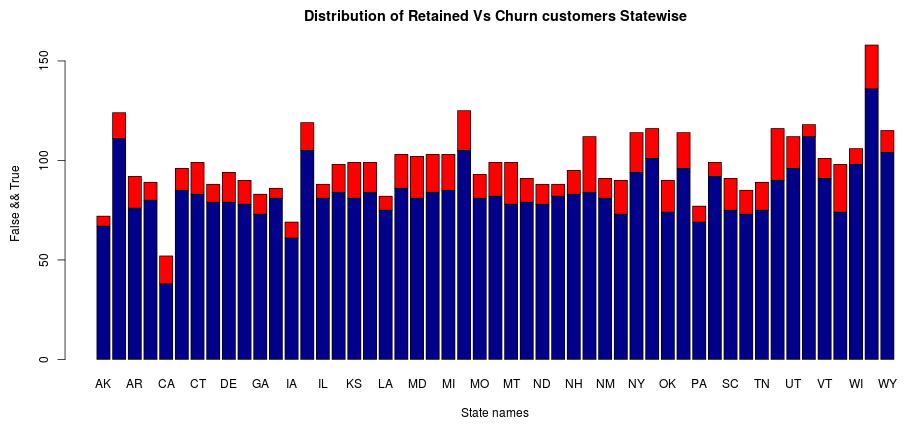
\includegraphics[width=10cm, height=6cm]{ppt_figures/web_dash_2}
	\end{figure}
\end{frame}

\begin{frame}
	\begin{figure}
		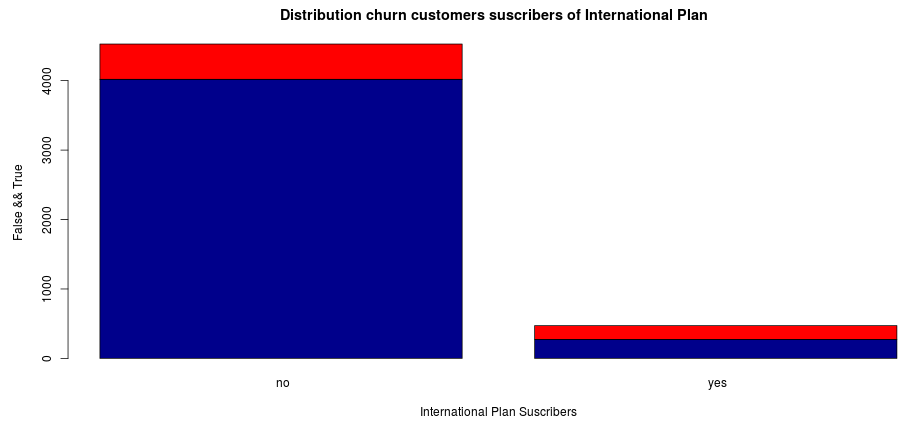
\includegraphics[width=10cm, height=6cm]{ppt_figures/web_dash_3}
	\end{figure}
\end{frame}

\end{document}

